\icode{N23S-EMI-SI-L2-261004-001}
\nceeID[4]{2023江苏}{8}
如图所示，圆形区域内有垂直纸面向里的匀强磁场，\(OC\)导体棒的\(O\)端位于圆心，棒的中点\(A\)位于磁场区域的边缘。现使导体棒绕\(O\)点在纸面内逆时针转动。\(O\)、\(A\)、\(C\)点电势分别为\(\varphi_O\) 、\(\varphi_A\)、\(\varphi_C\)，则\paren[A]

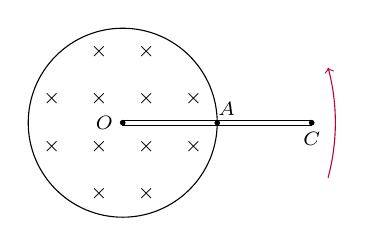
\begin{tikzpicture}[scale=.6,font=\scriptsize]
	\draw (0,0) circle(2);
	\draw (0,.05) rectangle(4,-.05);
	\foreach \x in {-1.5,-.5,...,1.5}
		\foreach \y in {-.5,.5}
		\node at(\x,\y) {\( \times \)};
	\foreach \y in {-1.5,1.5}
		\foreach \x in {-.5,.5}
		\node at(\x,\y) {\( \times \)};
	\foreach \x in {0,2,4}
		\fill (\x,0) circle(.06);
	\node at(0,0)[left]{\(O\)};
	\node at(4,0)[below]{\(C\)};
	\node at(2.2,.3){\(A\)};
	\draw[->,purple] (-15:4.5) arc(-15:15:4.5);
\end{tikzpicture}
\begin{choices}
	\item \(\varphi_O >\varphi_C\)
	\item \(\varphi_C >\varphi_A\)
	\item \(\varphi_O =\varphi_A\)
	\item \(\varphi_O - \varphi_A =\varphi_A -\varphi_C\)
\end{choices}
\begin{answer}
	A\qquad 提示：\(\varepsilon = \frac{1}{2}BL^2\omega\)
\end{answer}